\documentclass[border=2mm]{standalone}

\newcommand{\zero}[1]{ % #1 sarà la coordinata x di partenza per il gruppo
  \foreach \x in {0} {
    \filldraw[fill=white, opacity=0.5, draw=black,line width=0.4pt] (\x+#1,0) rectangle (\x+#1,1);
  }
  \draw[line width=0.8pt] (#1,0) rectangle (#1,1);
}

\newcommand{\uno}[1]{ % #1 sarà la coordinata x di partenza per il gruppo
  \foreach \x in {0} {
    \filldraw[fill=white, opacity=0.5, draw=black,line width=0.4pt] (\x+#1,0) rectangle (\x+1+#1,1);
  }
  \draw[line width=0.8pt] (#1,0) rectangle (1+#1,1);
}

\newcommand{\due}[1]{ % #1 sarà la coordinata x di partenza per il gruppo
  \foreach \x in {0,1} {
    \filldraw[fill=red, opacity=0.5, draw=black,line width=0.4pt] (\x+#1,0) rectangle (\x+1+#1,1);
  }
  \draw[line width=0.8pt] (#1,0) rectangle (2+#1,1);
}

\newcommand{\tre}[1]{ % #1 sarà la coordinata x di partenza per il gruppo
  \foreach \x in {0,1,2} {
    \filldraw[fill=green, opacity=0.5, draw=black,line width=0.4pt] (\x+#1,0) rectangle (\x+1+#1,1);
  }
  \draw[line width=0.8pt] (#1,0) rectangle (3+#1,1);
}

\newcommand{\quattro}[1]{ % #1 sarà la coordinata x di partenza per il gruppo
  \foreach \x in {0,1,2,3} {
    \filldraw[fill=magenta, opacity=0.5, draw=black,line width=0.4pt] (\x+#1,0) rectangle (\x+1+#1,1);
  }
  \draw[line width=0.8pt] (#1,0) rectangle (4+#1,1);
}

\newcommand{\otto}[1]{
  \foreach \i in {0,1} {
    \quattro{4*\i+#1};
  }
  \draw[line width=0.8pt] (#1,0) rectangle (8+#1,1);
}

\newcommand{\dodici}[1]{
  \foreach \i in {0,1,2} {
    \quattro{4*\i+#1};
  }
  \draw[line width=0.8pt] (#1,0) rectangle (12+#1,1);
}

\newcommand{\duepunti}[1]{
    \fill [black,opacity=1] (0.5+#1, 0.25) circle (2pt);
    \fill [black,opacity=1] (0.5+#1, 0.75) circle (2pt);
}

\newcommand{\uguale}[1]{
    \draw [black,opacity=1,line width=4pt] (0.15+#1, 0.25) -- (0.85+#1, 0.25);
    \draw [black,opacity=1,line width=4pt] (0.15+#1, 0.75) -- (0.85+#1, 0.75);
}

\newcommand{\piu}[1]{
    \draw [black,opacity=1,line width=4pt] (0.1+#1, 0.5) -- (0.9+#1, 0.5);
    \draw [black,opacity=1,line width=4pt] (0.5+#1, 0.1) -- (0.5+#1, 0.9);
}

\usepackage{tikz}

\begin{document}
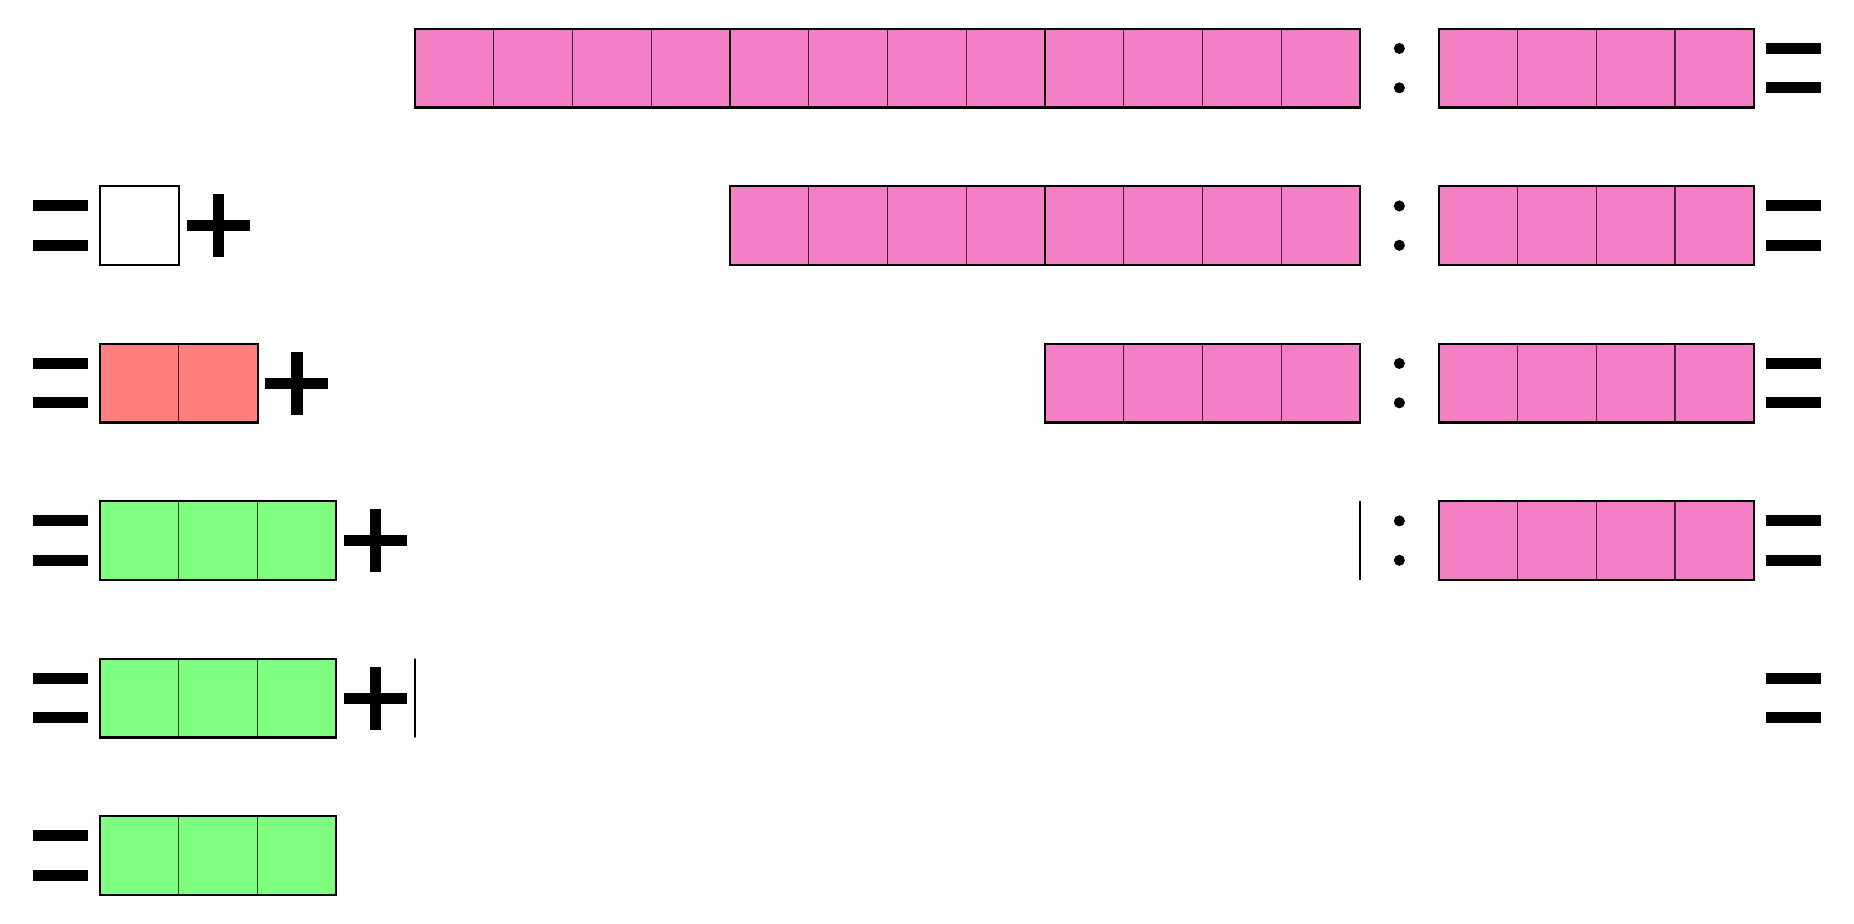
\begin{tikzpicture}[x=1cm, y=1cm]
    \begin{scope}[yshift=10cm]
        \dodici{5}
        \duepunti{17}
        \quattro{18}
        \uguale{22};
    \end{scope}

    \begin{scope}[yshift=8cm]
        \uguale{0}
        \uno{1}
        \piu{2}
        \otto{9}
        \duepunti{17}
        \quattro{18}
        \uguale{22};
    \end{scope}

    \begin{scope}[yshift=6cm]
        \uguale{0}
        \due{1}
        \piu{3}
        \quattro{13}
        \duepunti{17}
        \quattro{18}
        \uguale{22};
    \end{scope}

    \begin{scope}[yshift=4cm]
        \uguale{0}
        \tre{1}
        \piu{4}
        \zero{17}
        \duepunti{17}
        \quattro{18}
        \uguale{22};
    \end{scope}

    \begin{scope}[yshift=2cm]
        \uguale{0}
        \tre{1}
        \piu{4}
        \zero{5}
        \uguale{22};
    \end{scope}

    \begin{scope}[yshift=0cm]
        \uguale{0}
        \tre{1}
    \end{scope}
\end{tikzpicture}

\end{document}
